\section{Joined model method}
% Delete the text and write your Method(s) here:
%------------------------------------
In the subsequent section we shall in detail describe the method used to link the atmosphere and interior model. \Cref{tab:QOI} details the quantities that will be used.\par

\begin{table}[htb]%
\centering
\caption{Quantities of interest.}
	\label{tab:QOI}
	\begin{tabular}{ccc}
		\toprule
		Variable & {Exorem}  &  {Exoris}  \\
		\midrule
        \midrule
        Pressure & {$P_{rem}$}  &  {$P_{ris}$}  \\
        \midrule
		Temperature at 1bar & {$T_{rem}$}  &  {$T_{ris}$}  \\
        \midrule
		Mass at 1bar & {$M_{rem}$}  &  {$M_{ris}$}  \\
        \midrule
		Radius at 1bar & {$R_{rem}$}  &  {$R_{ris}$}  \\
        \midrule
		Gravity at 1bar & {$g_{rem}$}  &  {$g_{ris}$}  \\
        \midrule
		Molar mass at 1bar & {$\mu_{rem}$}  &  {$\mu_{ris}$}  \\
        \midrule
		Variable (X) at P & {$X_{rem}(P)$}  &  {$X_{ris}(P)$}  \\
        \midrule
		Internal temperature & {$T_{int}$}  &  {-}  \\
        \midrule
		Irradiation temperature & {$T_{irr}$}  &  {-}  \\
        \midrule
		{Variable (X) at $P_c$} & {$X_{rem-c}$}  &  {$X_{ris-c}$}  \\
        \midrule
		Convective region & {$P_c$}  &  {-}  \\
        \midrule
		Entropy & {-}  &  {$S$}  \\
        \midrule
		Core mass ratio & {-}  &  {$core$}  \\
        \midrule
		He/H fraction & {-}  &  {$\gamma_{he}$}  \\
		\bottomrule
	\end{tabular}
\end{table}

It is inherently hard to link very different models and a certain amount of choices and approximations need to be made, they are as follows :

\begin{itemize}
    \item Model linkage can only be done at pressures where the atmosphere is convective
    \item The mass of the atmosphere is considered negligible compared to that of the interior and core
    \item The atmosphere's mean molecular weight is reached in the interior by adjusting the He/H fraction
\end{itemize}

We also need to know what quantities absolutely need to be linked, they are as follows :

\begin{itemize}
    \item Pressure
    \item Temperature
    \item Molecular mass
    \item Gravity
\end{itemize}

One could expect it to be necessary to link the heat capacity ratio which is defined as follows :\par

\begin{align} 
    \frac{\partial ln(T)}{\partial ln(P)} = \frac{\gamma - 1}{\gamma} \Bigg|_{S} \label{eq:HC}
\end{align}

However as we are considering linking two models with different equations of state this is not deemed possible and also unnecessary. Indeed should pressure, temperature and molecular mass be equal then the heat ratio will be continuous too. (To be verified)\par

To guide the linkage a grid of both models is made over a range of input values, the grid is explicited in \cref{tab:Exorem} and \cref{tab:Exoris}

\begin{table}[htb]%
\centering
\caption{Exorem grid layout.}
	\label{tab:Exorem}
	\begin{tabular}{c}
		\toprule
		{$exorem(T_{int},T_{irr},g_{rem}) = T_{rem}(P), \mu_{rem}(P), P_c$}  \\
		\midrule
        \midrule
        $T_{irr} \in [0;1500] \, (K)$ \\
        \midrule
		$T_{int} \in [0;1000] \, (K)$   \\
        \midrule
		$g_{rem} \in [2;100] \, (m/s^2)$   \\
        \bottomrule
	\end{tabular}
\end{table}

\begin{table}[htb]%
\centering
\caption{Exoris grid layout.}
	\label{tab:Exoris}
	\begin{tabular}{c}
		\toprule
		{$exoris(T_{ris},core,\gamma_{he/h}, M) = S, R_{rem}$}  \\
		\midrule
        \midrule
        {$T_{ris} \in [150;1500] \, (K)$} \\
        \midrule
		{$core = 10 \, M_{e}$}   \\
        \midrule
		{$\gamma_{he} \in [0.1;0.5]$}   \\
        \midrule
		{$M \in [0.1;15] \, (M_J)$}   \\
        \bottomrule
	\end{tabular}
\end{table}


Given grid parameters depend on the capacity of the models to converge correctly, low temperature inputs can lead to non converged solutions. \par

\begin{figure}
    \centering
    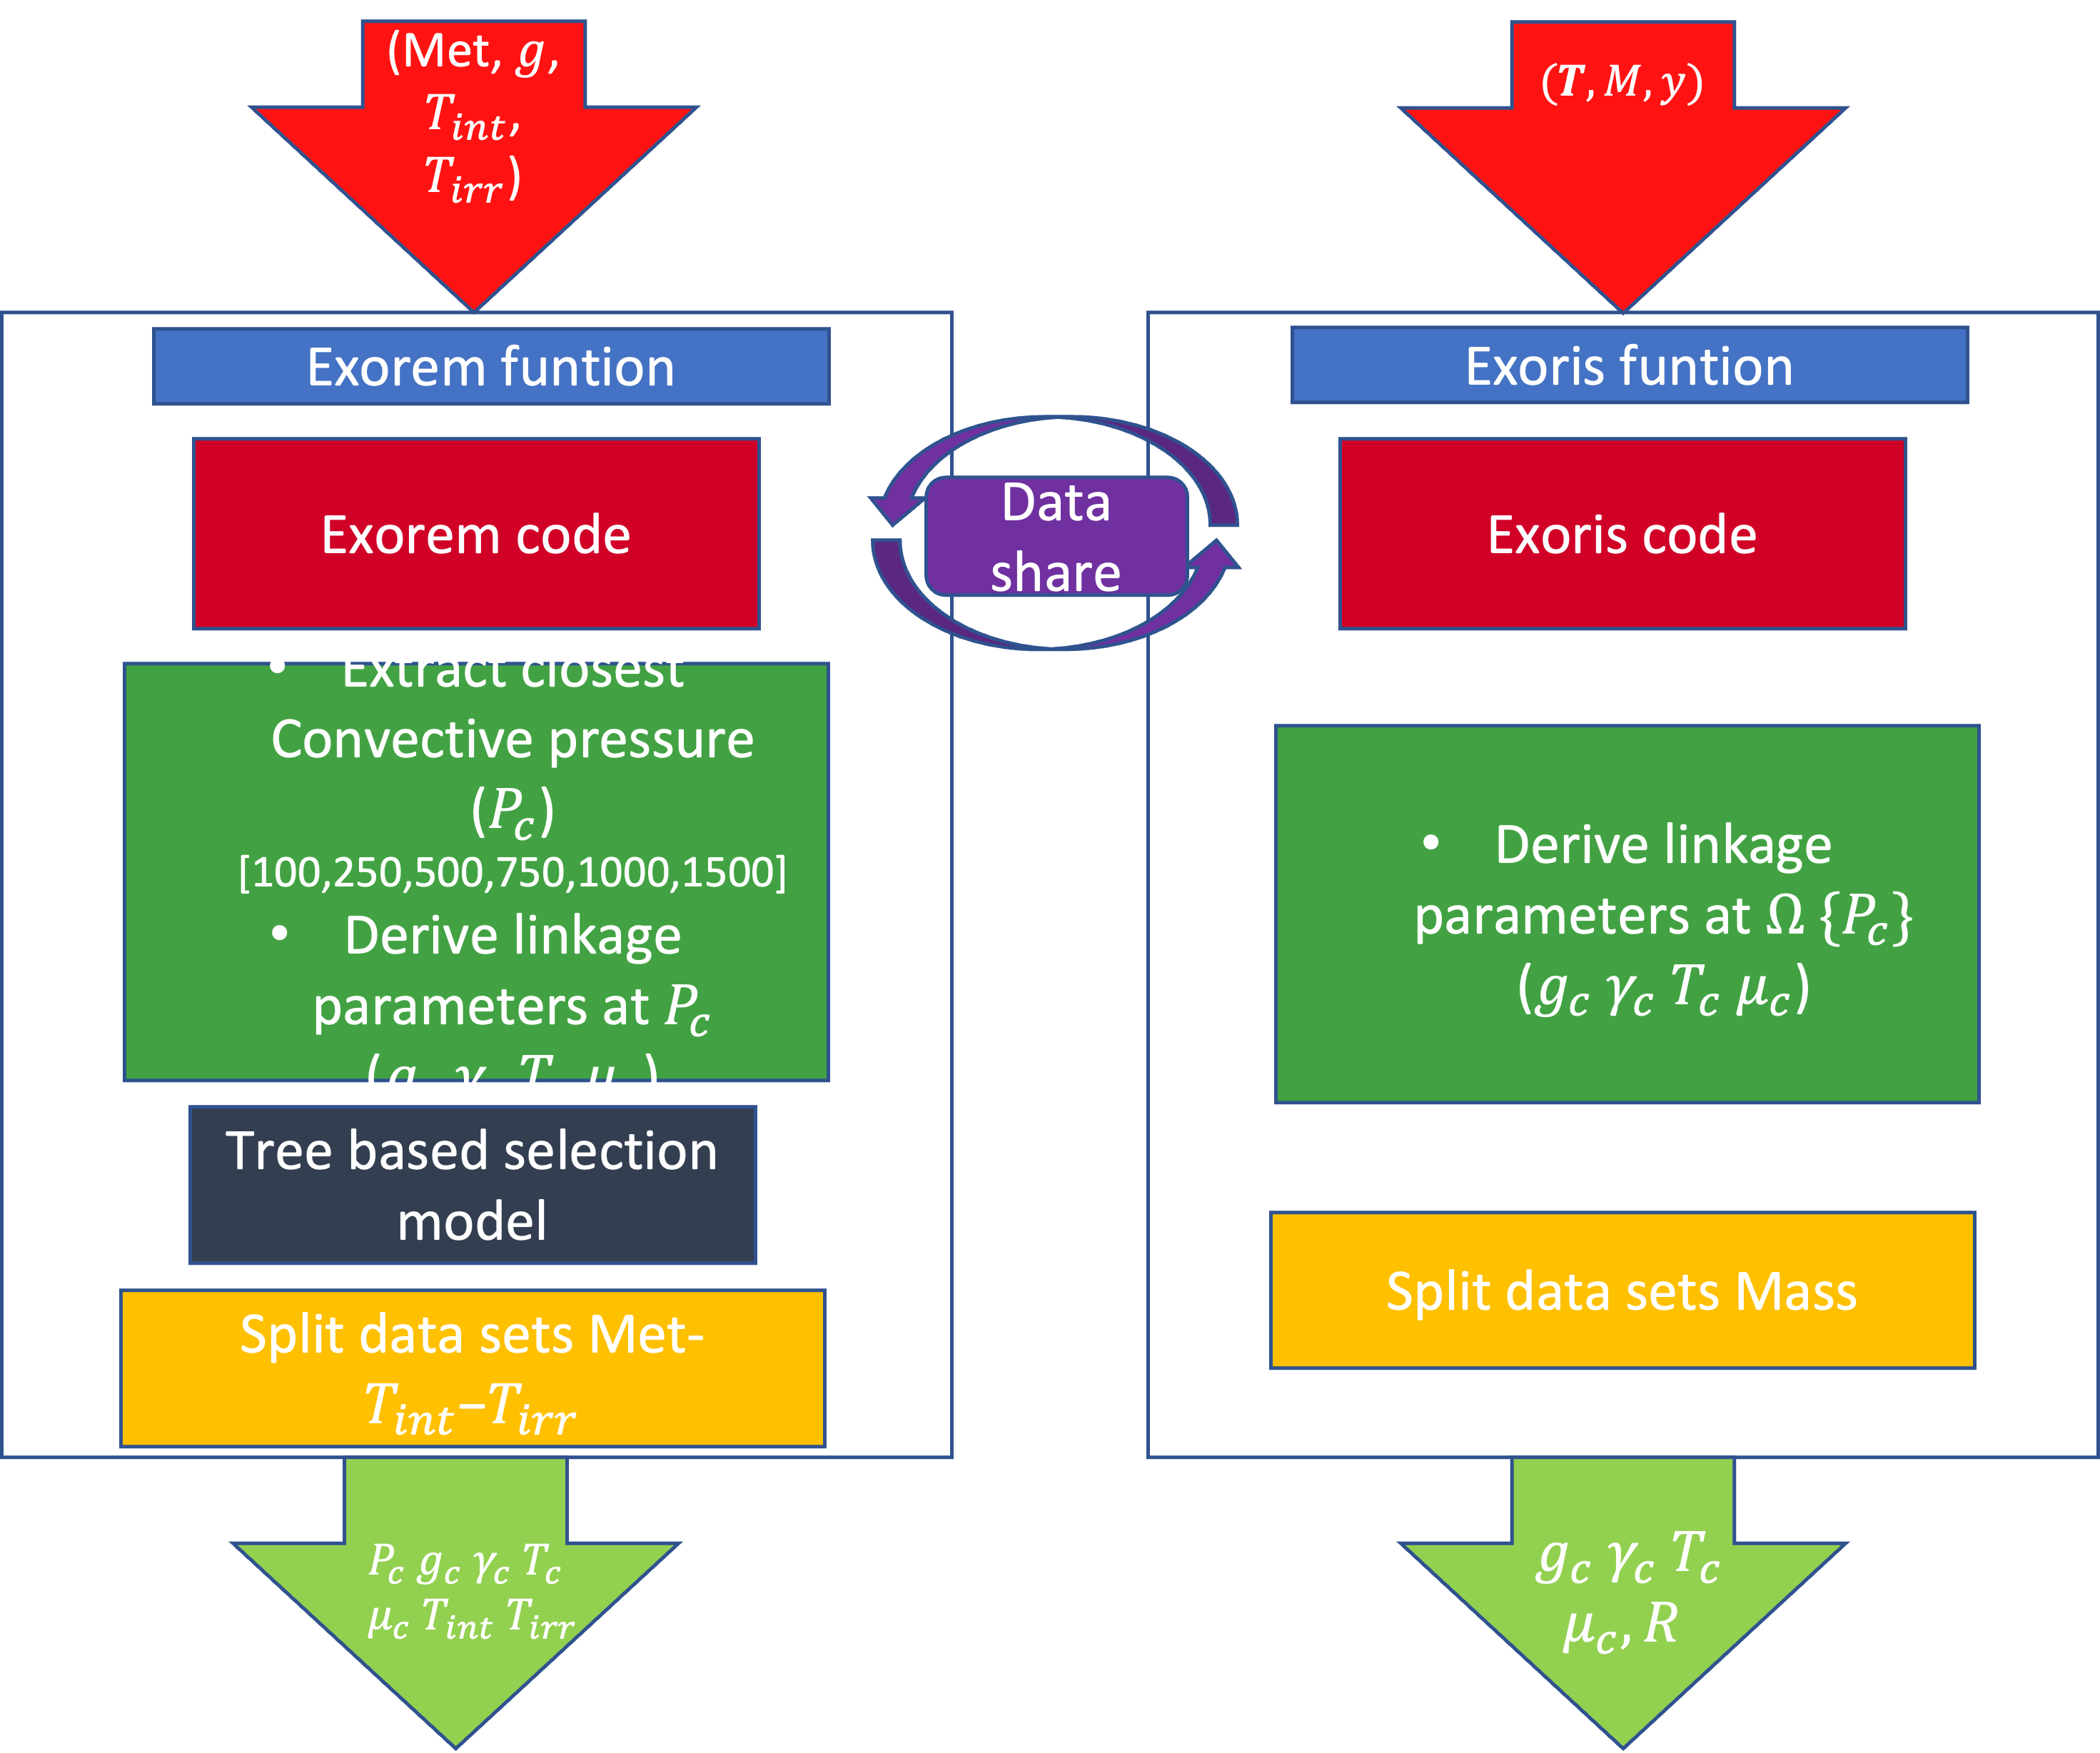
\includegraphics[width=0.48\textwidth]{Images/grid_model_function.png}
    \caption{Organigram of how Exoris and Exorem are packaged into grid functions.}
    \label{fig:Exoris_Exorem_grid_functions}
\end{figure}

\Cref{fig:Exoris_Exorem_grid_functions} details how exorem and exoris grids are in practice made. To help subsequent steps, there is a small level of grid sharing on tempereature values between exorem and exoris. This is to make sure that the grids overlap. Exorem can struggle to converge at low irradiation temperatures for high internal temperatures. A non grey analytical model from Guillot \parencite{guillot_radiative_2010} is used in these regions to initialise exorem with pressure temperature profiles. However, this is often not sufficient, as such, a basic tree based machine learning model is trained to remove improperly converged pressure-temperature profiles, further details can be found in the anexes. \par

Linkage between models is always carried out for the pressures where Exorem is convective, this adds a certain level of complexity to the problem. Indeed to minimize the effect of the non-precise ideal gas law used in exorem, we want to link at the lowest possible pressure as such at the point where the atmosphere has started exhibiting a convective behaviour. We hence need to interpolate the exoris quantities to this pressure. In practice we avoid doing this as it would be computationally tiresome and would lead to the size of the exoris grid being multiplied by the size of the exorem one. As such the convective pressures for all the exorem grid values are grouped into a bins of convective pressures. These bins are 100, 250, 500, 750, 1000 and 1500 bars, the bin is chosen as to always be of a superior value to the real convective pressure as to insure that the atmosphere is indeed convective. \par

Using the grids as a guide, the linkage is done via iterative calling of the exorem and exoris code. As shown in \cref{fig:Exoris_Exorem_grid_functions} we split the grids into $T_{int}$ and $T_{irr}$ sub grids for exorem and $M_{ris}$ subgrids for exoris. Hence the process outlined in \cref{fig:Iterative_process} is undertaken for a user chosen ($T_{int}$,$T_{irr}$,$M_{ris}$,$core$) where $M_{ris}$ will become the chosen planatary $M$ for which we wish to determine the properties such as the radius ($Req$), spectra ($J_{rad}$), effective temperature ($T_{eff}$) and entropy ($S$).\par

\begin{figure}
    \centering
    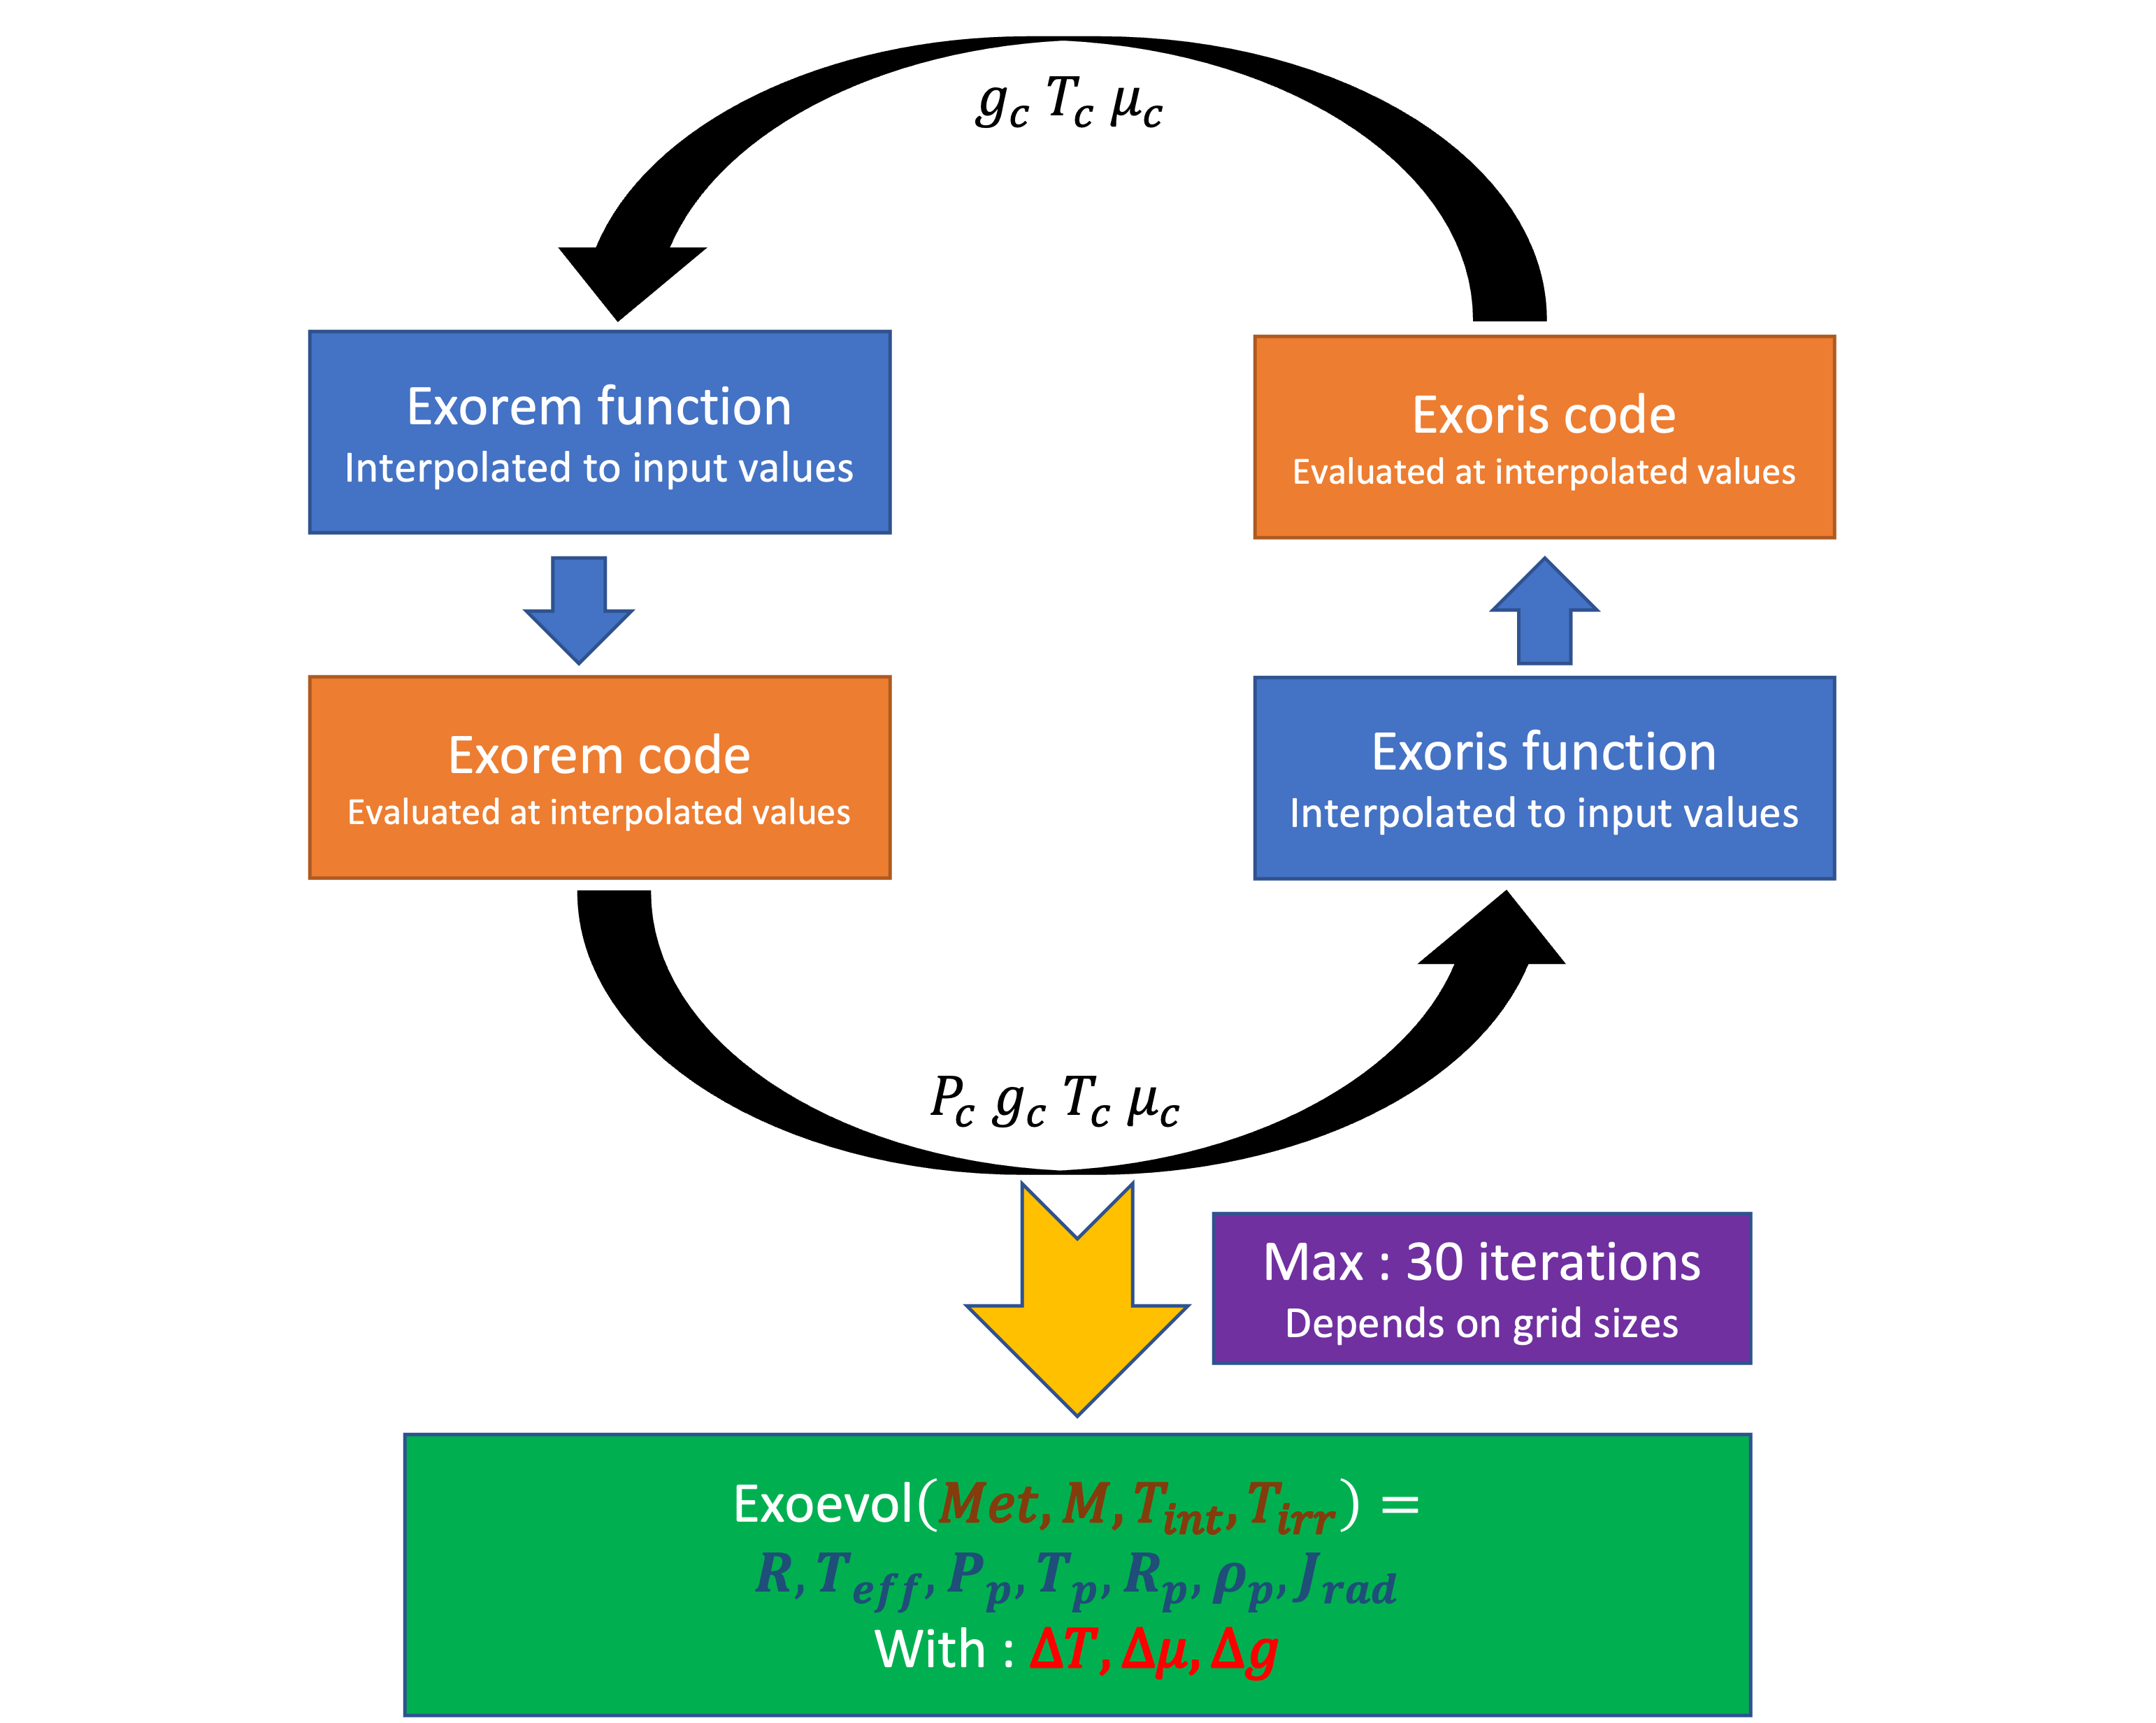
\includegraphics[width=0.48\textwidth]{Images/Iterative_process.png}
    \caption{Iterative process to converge exorem and exoris models}
    \label{fig:Iterative_process}
\end{figure}

The objective of this iterative process is to reduce the erreur on the three quantities to link below a certain threshold. This threshold is determined a posteriori as to find the right balance between convergence time and precision.\par

It is worth detailing the interpolation method in order to understand better the steps completed during an iteration. Interpolation in high dimensional space poses notable challenges. Indeed points can be distant from one another and desired points can be badly surrounded by grid values. It is important to know the layout of the variables and what we want to obtain. Using the details from \cref{tab:Exorem} and \cref{tab:Exoris}, we see the input and output variables. Input variables are always given at a pressure of 1 bar and output variables at the linkage pressure ($P_c$). As such as stated, before running the iterative procedure including interpolations, we have fixed ($T_{int}$,$T_{irr}$,$M_{ris}$,$core$). We hence need to find at each step ($g_{rem}$,$T_{ris}$,$\gamma_{he}$) from the values obtained at the linkage pressure ($P_c$,$T_c$,$\mu_c$,$g_c$). We will seperate the cases between exorem and exoris.\par

For exorem, we uniquely need to find the equatorial gravity at 1bar, to do this a simple plotting of how the surface gravity varies with the given parameters shows the following :

\begin{align} 
    g_s = f(P_c,T_c,\mu_c,g_c) = f(P_c, g_c) \overset{\mathrm{at \, P_c}}{=} ag_c + b \\
    (a,b) \in (R,R) \nonumber
\end{align}

As such we use a simple linear regression. We avoid all extrapolations. As such, should the value of $g_c$ not be included in the grid, then an exploration is undertaken as to include it. This can be the case for large mass planets.\par

For exoris, we need to find $T_{ris}$ and $\gamma_{he}$. To do this we chose to fix the input value of $\gamma_{he}$ using the average molecular mass ($\mu_c$) using the following :

\begin{align} 
    \frac{1}{\mu} = (1-\gamma_{he})\frac{1}{\mu_{h_2}} + \gamma_{he}*\frac{1}{\mu_{he}}
\end{align}

Which gives $\gamma_{he}$ :

\begin{align} 
    \gamma_{he} = 2-\frac{4}{\mu}
\end{align}

We can now look for the surface pressure to use in exoris ($T_{ris}$). To do this, we again plot its behaviour against the given parameters at $P_c$ this shows the following :

\begin{align} 
    T_{ris} = f(P_c,T_c,\mu_c,g_c) \overset{\mathrm{at \, P_c}}{=} f(T_c,\mu_c,g_c)
\end{align}

Indeed this represents a certain challenge as $T_{ris}$ is the result of a combination of all the parameters. We hence have to interpolate in a four dimensional space. To do this we propose to use a barycentric interpolation using a Delaunay triangulation, the full description of this method is given in the annexes. From a practical standpoint, this method requires the desired point to be contained within a triangle (pyramid in 3d). Either this is already the case with the guiding grid and a point within the triangle can be found, or this is not the case and an exploration is required to build the surrounding values. It is uncertain how smooth the space included within the triangulation values is. As such multiple iterations of interpolation and exoris model running are required in order to find the point of interest within a given tolerance. \par

These interpolation and model running steps are shown in \cref{fig:Iterative_process}. More work is required for the interpolations, most notably how to find surrounding values efficiently.

(Image showing convergence evolution required here)